%=============================================================================
% File:  ex_complex_01.tex --  tikz-network example
% Author(s): Jürgen Hackl <hackl@ibi.baug.ethz.ch>
% Creation:  20 Sep 2017
% Time-stamp: <Mit 2017-09-20 15:04 juergen>
%
% Copyright (c) 2017 Jürgen Hackl <hackl@ibi.baug.ethz.ch>
%               http://www.ibi.ethz.ch
% $Id$
%
% More information on LaTeX: http://www.latex-project.org/
% LaTeX symbol list: 
%   http://www.ctan.org/tex-archive/info/symbols/comprehensive/symbols-a4.pdf
%=============================================================================
\documentclass{standalone}

% Used packages
\usepackage{../../tikz-network}

\begin{document}


\tikzset{every picture/.style={line width=0.75pt}} %set default line width to 0.75pt        

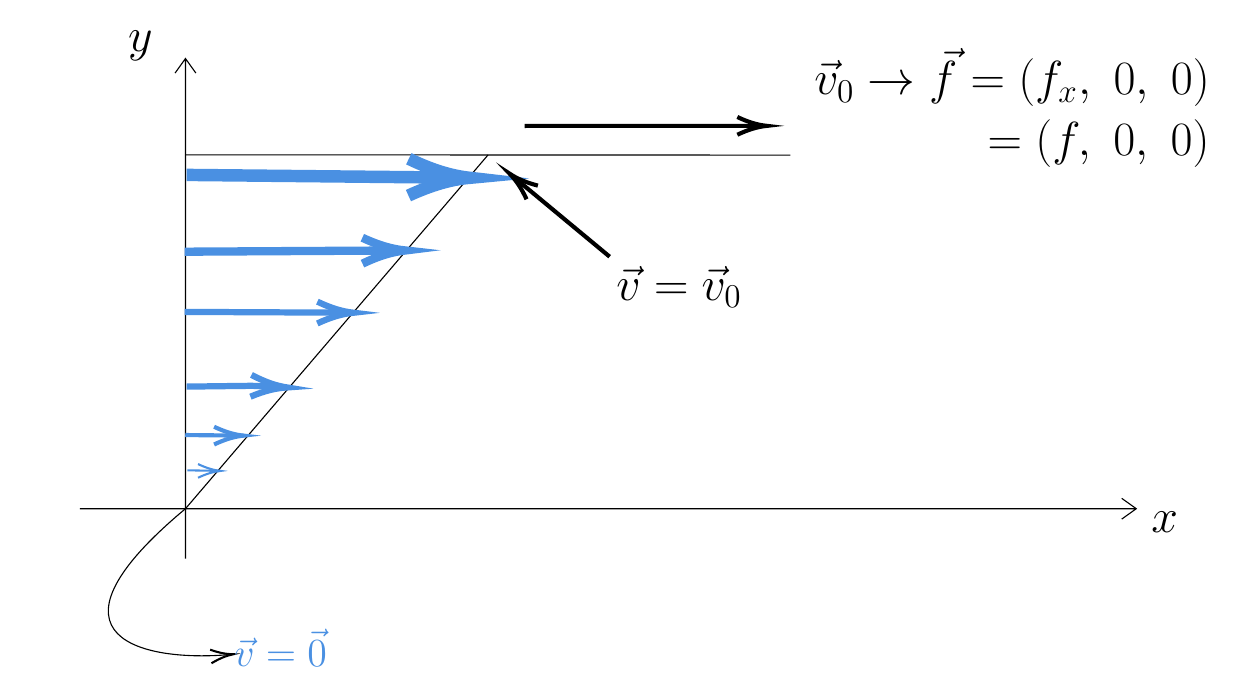
\begin{tikzpicture}[x=0.75pt,y=0.75pt,yscale=-1,xscale=1]
%uncomment if require: \path (0,354); %set diagram left start at 0, and has height of 354

%Shape: Axis 2D [id:dp5437489803461968] 
\draw  (59,240.5) -- (568,240.5)(109.9,23.6) -- (109.9,264.6) (561,235.5) -- (568,240.5) -- (561,245.5) (104.9,30.6) -- (109.9,23.6) -- (114.9,30.6)  ;
%Straight Lines [id:da9192039699134926] 
\draw    (110,70) -- (401.36,70.12) ;
%Straight Lines [id:da06062171121825255] 
\draw    (109.9,240.5) -- (255.68,70.06) ;
%Straight Lines [id:da8174566828306293] 
\draw [color={rgb, 255:red, 74; green, 144; blue, 226 }  ,draw opacity=1 ][line width=4.5]    (110.47,79.67) -- (239.93,80.99) ;
\draw [shift={(246.93,81.07)}, rotate = 180.59] [color={rgb, 255:red, 74; green, 144; blue, 226 }  ,draw opacity=1 ][line width=4.5]    (29.51,-8.88) .. controls (18.76,-3.77) and (8.93,-0.81) .. (0,0) .. controls (8.93,0.81) and (18.76,3.77) .. (29.51,8.88)   ;
%Straight Lines [id:da6518144753858666] 
\draw [color={rgb, 255:red, 74; green, 144; blue, 226 }  ,draw opacity=1 ][line width=3]    (109.47,116.67) -- (210.93,116.09) ;
\draw [shift={(215.93,116.07)}, rotate = 179.68] [color={rgb, 255:red, 74; green, 144; blue, 226 }  ,draw opacity=1 ][line width=3]    (20.77,-6.25) .. controls (13.2,-2.65) and (6.28,-0.57) .. (0,0) .. controls (6.28,0.57) and (13.2,2.66) .. (20.77,6.25)   ;
%Straight Lines [id:da6555246590269845] 
\draw [color={rgb, 255:red, 74; green, 144; blue, 226 }  ,draw opacity=1 ][line width=2.25]    (109.47,145.67) -- (186.93,146.05) ;
\draw [shift={(190.93,146.07)}, rotate = 180.28] [color={rgb, 255:red, 74; green, 144; blue, 226 }  ,draw opacity=1 ][line width=2.25]    (17.49,-5.26) .. controls (11.12,-2.23) and (5.29,-0.48) .. (0,0) .. controls (5.29,0.48) and (11.12,2.23) .. (17.49,5.26)   ;
%Straight Lines [id:da48728258324316287] 
\draw [color={rgb, 255:red, 74; green, 144; blue, 226 }  ,draw opacity=1 ][line width=2.25]    (110.47,181.67) -- (141.91,181.28) -- (154.94,181.88) ;
\draw [shift={(158.93,182.07)}, rotate = 182.65] [color={rgb, 255:red, 74; green, 144; blue, 226 }  ,draw opacity=1 ][line width=2.25]    (17.49,-5.26) .. controls (11.12,-2.23) and (5.29,-0.48) .. (0,0) .. controls (5.29,0.48) and (11.12,2.23) .. (17.49,5.26)   ;
%Straight Lines [id:da8523463443270776] 
\draw [color={rgb, 255:red, 74; green, 144; blue, 226 }  ,draw opacity=1 ][line width=1.5]    (109.8,205) -- (137.91,205.28) ;
\draw [shift={(137.91,205.28)}, rotate = 180] [color={rgb, 255:red, 74; green, 144; blue, 226 }  ,draw opacity=1 ][line width=1.5]    (14.21,-4.28) .. controls (9.04,-1.82) and (4.3,-0.39) .. (0,0) .. controls (4.3,0.39) and (9.04,1.82) .. (14.21,4.28)   ;
%Straight Lines [id:da19627653067167983] 
\draw [color={rgb, 255:red, 74; green, 144; blue, 226 }  ,draw opacity=1 ][line width=0.75]    (110.8,222) -- (126.91,222.28) ;
\draw [shift={(126.91,222.28)}, rotate = 180] [color={rgb, 255:red, 74; green, 144; blue, 226 }  ,draw opacity=1 ][line width=0.75]    (10.93,-3.29) .. controls (6.95,-1.4) and (3.31,-0.3) .. (0,0) .. controls (3.31,0.3) and (6.95,1.4) .. (10.93,3.29)   ;
%Straight Lines [id:da7369240862978534] 
\draw [line width=1.5]    (314.27,119.07) -- (268.35,80.96) ;
\draw [shift={(266.04,79.04)}, rotate = 39.69] [color={rgb, 255:red, 0; green, 0; blue, 0 }  ][line width=1.5]    (14.21,-4.28) .. controls (9.04,-1.82) and (4.3,-0.39) .. (0,0) .. controls (4.3,0.39) and (9.04,1.82) .. (14.21,4.28)   ;
%Straight Lines [id:da8649686616934051] 
\draw [line width=1.5]    (273.27,56.07) -- (387,56.04) ;
\draw [shift={(390,56.04)}, rotate = 179.99] [color={rgb, 255:red, 0; green, 0; blue, 0 }  ][line width=1.5]    (14.21,-4.28) .. controls (9.04,-1.82) and (4.3,-0.39) .. (0,0) .. controls (4.3,0.39) and (9.04,1.82) .. (14.21,4.28)   ;
%Curve Lines [id:da08930815555372273] 
\draw    (109.9,240.5) .. controls (34.15,303.64) and (91.23,314.29) .. (131.19,310.77) ;
\draw [shift={(133,310.6)}, rotate = 174.29] [color={rgb, 255:red, 0; green, 0; blue, 0 }  ][line width=0.75]    (10.93,-3.29) .. controls (6.95,-1.4) and (3.31,-0.3) .. (0,0) .. controls (3.31,0.3) and (6.95,1.4) .. (10.93,3.29)   ;

% Text Node
\draw (574,241) node [anchor=north west][inner sep=0.75pt]  [font=\LARGE] [align=left] {$\displaystyle x$};
% Text Node
\draw (81,9) node [anchor=north west][inner sep=0.75pt]  [font=\LARGE] [align=left] {$\displaystyle y$};
% Text Node
\draw (405,17.4) node [anchor=north west][inner sep=0.75pt]  [font=\LARGE]  {$ \begin{array}{l}
\vec{v}_{0}\rightarrow \vec{f} =( f_{x} ,\ 0,\ 0)\\
\ \ \ \ \ \ \ \ \ \ \ \ =( f,\ 0,\ 0)
\end{array}$};
% Text Node
\draw (316.27,122.47) node [anchor=north west][inner sep=0.75pt]  [font=\LARGE]  {$\vec{v} =\vec{v}_{0}$};
% Text Node
\draw (132.27,297.47) node [anchor=north west][inner sep=0.75pt]  [font=\Large,color={rgb, 255:red, 74; green, 144; blue, 226 }  ,opacity=1 ]  {$\vec{v} =\vec{0}$};


\end{tikzpicture}
\end{document}
%=============================================================================
% eof
%
% Local Variables:
% mode: latex
% mode: linum
% mode: auto-fill
% fill-column: 80
% TeX-master: t
% End:
